\documentclass[10pt,dvipsnames]{beamer}
\mode<beamer>{%
	%\usetheme{Ilmenau}
	%\usetheme[compress]{Ilmenau}
	\usetheme{CambridgeUS}
}

%\setbeamertemplate{mini frames}[tick]
\setbeamertemplate{navigation symbols}{}
\setbeamertemplate{footline}[frame number]{}

%\usepackage[brazil]{babel}   
\usepackage[utf8]{inputenc}
\usepackage[T1]{fontenc}
\usepackage{todonotes}
%\usepackage{tikz}		% para fazer diagramas

%\usepackage{classicthesis}

\usepackage{booktabs}	% for better rules in tables

\usepackage{tabularx} % better tables
    \setlength{\extrarowheight}{3pt} % increase table row height
\newcommand{\tableheadline}[1]{\multicolumn{1}{c}{\spacedlowsmallcaps{#1}}}
\newcommand{\myfloatalign}{\centering} % to be used with each float for alignment

\DeclareGraphicsExtensions{.pdf,.jpg,.png} % compilamos apenas com pdflatex
\graphicspath{{./gfx/}} % caminho onde as figuras estarao disponiveis

\newcommand{\myspacing}{\itemsep2ex}

\title{Information Retrieval from Clinical Reports}
\author{Michel Oleynik}
\institute[Medical University of Graz, Austria]{
Institute for Medical Informatics, Statistics and Documentation\\
Medical University of Graz, Austria
}
\titlegraphic{
\includegraphics[width=15mm]{medunigraz-small.jpg}}
\date{2016}

\newcommand*\oldmacro{}%
\let\oldmacro\insertshorttitle%
\renewcommand*\insertshorttitle{%
  \oldmacro\hfill%
  \insertframenumber\,/\,\inserttotalframenumber}

\begin{document}

\begin{frame}
	\titlepage
\end{frame}

%=================================================================
%\input{slides-introduction}

%=================================================================
%\section{Agenda}

%\begin{frame}
%\frametitle{Agenda}
%\tableofcontents[hideallsubsections]
%\end{frame}

%\AtBeginSection[] % Do nothing for \section*
%{
%\begin{frame}<beamer>
%\frametitle{Outline}
%\tableofcontents[currentsection,hideallsubsections]
%\end{frame}
%}

%=================================================================
%=================================================================
\section*{Motivation}

%-----------------------------------------------------------------
%\subsection{This is a subsection}
\begin{frame}
	\frametitle{Motivation}
	\begin{itemize} \myspacing
		\item Huge amount of clinical data produced over the years
		\item Different content types
		\begin{itemize}
			\item Unstructured and semi-structured texts
			\item Numeric and coded data
			\item Biosignals and images
		\end{itemize}
		\item Clinical text
		\begin{itemize}
			\item Short forms: abbreviations, acronyms
			\item Spelling and typing errors
			\item Short, incomplete sentences
		\end{itemize}
		\item Two problems addressed 
		\begin{itemize}
			\item Unsupervised expansion of ad-hoc abbreviations in EHR narratives
			\item Automated classification of pathology reports into ICD-O codes 
		\end{itemize}
	\end{itemize}
\end{frame}

%\begin{frame}
%	\frametitle{Motivation}
%                \begin{figure}
%        			\centering
%        			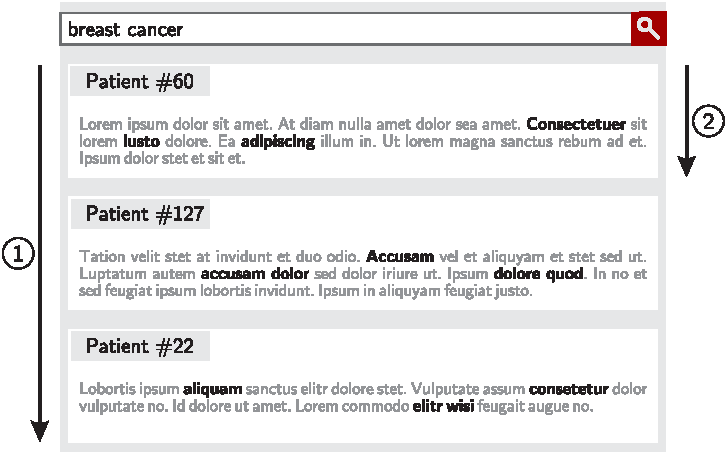
\includegraphics[width=10cm]{research_questions.pdf}
%        			\caption{Two research questions.}
%        			\label{fig:research_questions}
%  		\end{figure}
%\end{frame}

%=================================================================
%\section{Unsupervised expansion of ad-hoc abbreviations in EHR narratives}
\section{Goal}

%-----------------------------------------------------------------
%\subsection{Goal}

\begin{frame}
	\frametitle{1\textsuperscript{st} problem: abbreviation expansion}
	\begin{exampleblock}{Original}
	3. St.p. TE eines exulz. sek.knot.SSM (C43.5) li Lab. majus.\\
	Level IV, 2,42 mm Tumordurchm.
	\end{exampleblock}
	
	\pause
	
	\begin{exampleblock}{Expanded}
	Status post Totalexzision eines exulzerierenden sekundär knotigen superfiziell\\
	spreitenden Melanoms (C43.5) linkes Labium majus.\\
	Level Vier, 2,42 Millimeter Tumordurchmesser.
	\end{exampleblock}
	
	\pause
	
	\begin{exampleblock}{English translation}
	3. History of total excision of an exulcerated secondarily nodular superficially\\
	spreading melanoma (C43.5) of the outer left labia.\\
	Level 4, tumor diameter 2.42mm.
	\end{exampleblock}
\end{frame}

%\begin{frame}
%	\frametitle{Goal}
%	\begin{itemize} \myspacing
%		\item Unsupervised expansion of ad-hoc abbreviations in clinical narratives\footnotemark
%		\begin{itemize}
%			\item Unsupervised: no time/resources to train the system
%			\item Expansion: solve ambiguities
%			\item Ad-hoc: not in a dictionary
%			%\item EHR: Electronic Health Record
%			\item Narratives: free-text, no extra information available
%		\end{itemize}
%	\end{itemize}
%	\footnotetext[1]{Contribution to CBmed Project 1.2 (IICCAB)}
%\end{frame}

%=================================================================
%\section{Unsupervised expansion of ad-hoc abbreviations in EHR narratives}
\section{Materials and Methods}

%-----------------------------------------------------------------
%\subsection{Materials and Methods}

\begin{frame}
	\frametitle{Materials and Methods}
	\begin{itemize} \myspacing
		\item 30,000 clinical documents from the cardiology domain
		\begin{itemize}
			\item Written in German by Austrian physicians
			\item Discharge summaries, finding reports        
                         \item Routine documentation in LKH, Graz
                \end{itemize}

	\end{itemize}
\end{frame}

\begin{frame}
	\frametitle{Materials and Methods}
                \begin{figure}
        			\centering
        			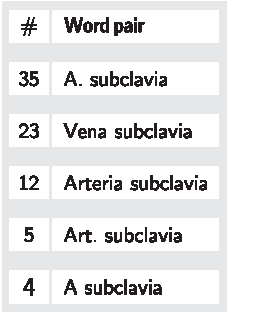
\includegraphics[height=5cm]{bigram.pdf}
        			\caption{Building a bigram (word pair) list.}
        			\label{fig:bigram_extraction}
  		\end{figure}
\end{frame}

\begin{frame}
	\frametitle{Materials and Methods}
                \begin{figure}
        			\centering
        			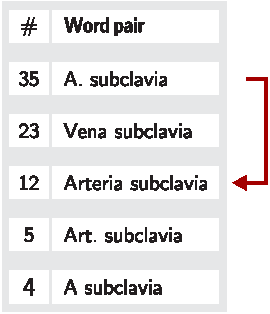
\includegraphics[height=5cm]{bigram_lookup.pdf}
        			\caption{Lookup in a bigram (word pair) list.}
        			\label{fig:bigram_lookup}
  		\end{figure}
\end{frame}

\begin{frame}
	\frametitle{Materials and Methods}
	\begin{itemize} \myspacing
	        \item Evaluation data
                \begin{itemize}
                		\item 200 random text excerpts centered on an abbreviation
			\item 147 abbreviations manually expanded by a human annotator
                \end{itemize}
%                \item ``Big data'': extract knowledge from available data
%                \begin{itemize}
%	                \item Unsupervised machine learning
%	                \item Training-test split (90\% - 10\%)
%		        \item Bigram (word pair) list lookup
%                \end{itemize}
	        \item Evaluation method
                \begin{itemize}
                		\item Recall (R): sensitivity
			\item Precision (P): positive predictive value
			\item $F$-score ($F_1$): harmonic mean of precision and recall
                \end{itemize}
	\end{itemize}
\end{frame}

%-----------------------------------------------------------------



%=================================================================
%\section{Unsupervised expansion of ad-hoc abbreviations in EHR narratives}

%-----------------------------------------------------------------
%\subsection{Materials and Methods}

\begin{frame}
	\frametitle{Partial Results\footnotemark}
\begin{table}[htbp]
	%\tiny
    	%\scriptsize
    	\footnotesize
    	%\small
	\caption{Precision, recall and $F$-score in different matching strategies.}
	\myfloatalign
    \begin{tabular}{lccccc}
    \toprule
	{\bf Matching} & {\bf N-Gram} &  {\bf P} & {\bf R} & {\bf $F_1$} \\
	\midrule
	Relaxed & 1 & 0.62 & 0.62 & 0.62 \\
	Strict & 1 & 0.76 & 0.71 & 0.74 \\
	Relaxed & 2 & 0.91 & 0.81 & 0.86 \\
	Strict & 2 & 0.94 & 0.73 & 0.82 \\
	Relaxed & 3 & 0.63 & 0.16 & 0.26 \\
	Strict & 3 & 0.91 & 0.20 & 0.32 \\
	\midrule
	{\bf Combined} & {\bf -} & {\bf 0.93} & {\bf 0.93} & {\bf 0.93} \\
	\bottomrule
    \end{tabular}
  \label{tab:abbreviation_metrics}
\end{table}
	\footnotetext[1]{Submitted to the 16th World Congress on Medical and Health Informatics [Medinfo 2017]}
\end{frame}

%-----------------------------------------------------------------


%%=================================================================
\section{Automated classification of pathology reports into ICD-O codes}

%-----------------------------------------------------------------
%\subsection{Goal}

\begin{frame}
	\frametitle{Goal}
	\begin{figure}
		\centering
		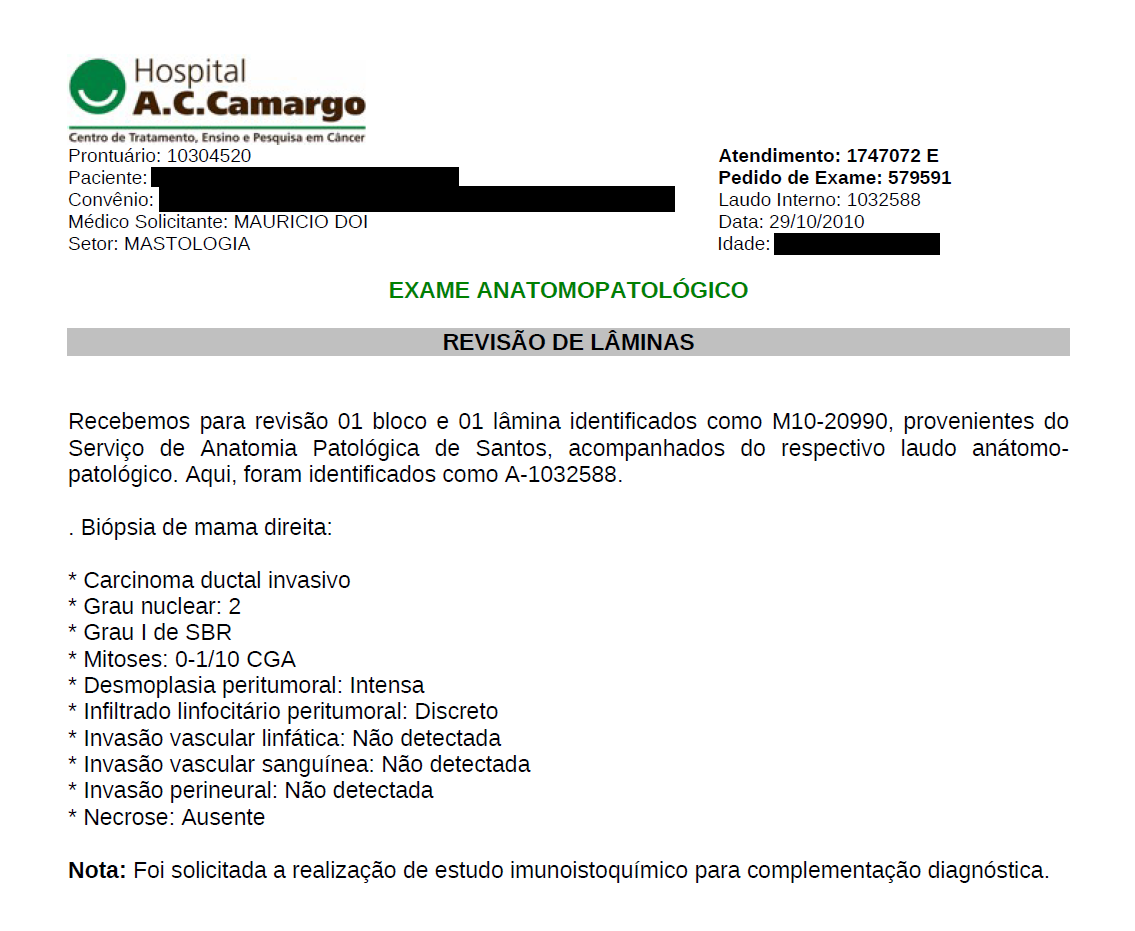
\includegraphics[height=7cm]{laudo-zoom.png}
		\caption{Example of a pathology report mapped into ICD-O codes.}
		\label{fig:laudo} 
	\end{figure}
\end{frame}

%%=================================================================
%\section{Automated classification of pathology reports into ICD-O codes}

%-----------------------------------------------------------------
%\subsection{Materials and Methods}

\begin{frame}
	\frametitle{Materials and Methods}
	\begin{itemize} \myspacing
		\item 70,000+ documents from 20,000+ patients over 14 years
		\begin{itemize}
			\item Written in Portuguese by Brazilian pathologists
			\item Pathology reports        
                         \item Routine procedure in A.C. Camargo Cancer Center, Brazil
                \end{itemize}
                 \item Gold standard creation
                \begin{itemize}
                		\item Free-text content associated to structured data in cancer registries
			\item Discarded patients with confirmed metastasis or multiple classifications
                \end{itemize}
                \item Supervised machine learning
                \begin{itemize}
			\item Micro-averaged with 10-fold cross-validation
			\item Evaluated by precision, recall and $F$-score
			\item Support vector machines (SVMs) with \emph{tf-idf} weighting scheme
			\begin{equation}
				\label{eq:svm}
				f(\vec{x}) = sign(\vec{w}^T\vec{x} + b)
			\end{equation}
                \end{itemize}

	\end{itemize}
\end{frame}

\begin{frame}
	\frametitle{Materials and Methods}
                \begin{figure}
        			\centering
        			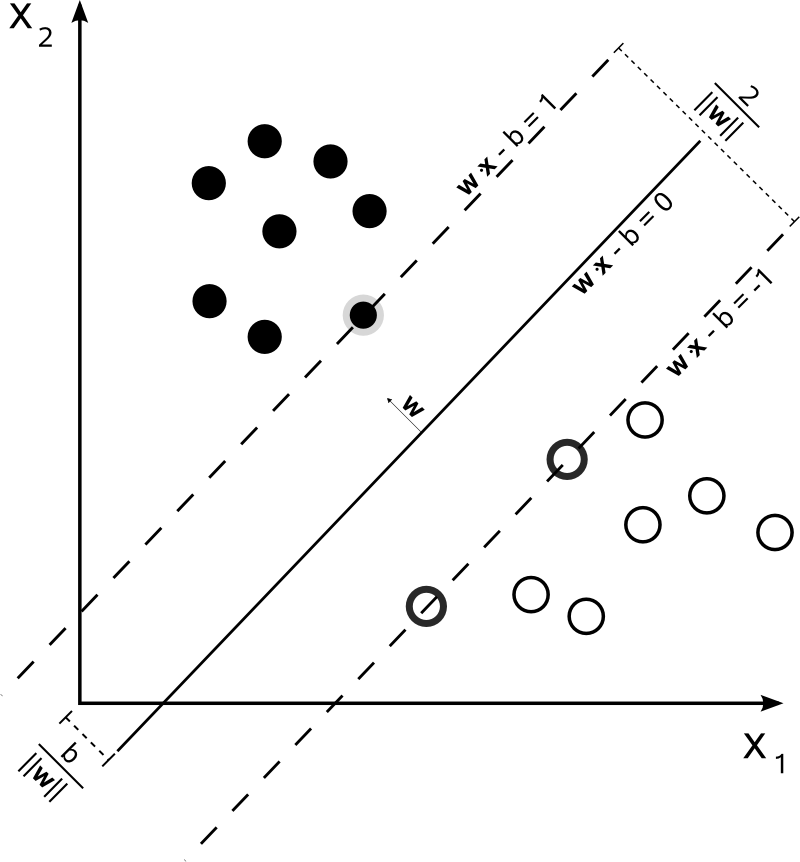
\includegraphics[width=6cm]{svm.png}
        			\caption{A support vector machine. [Public domain]}
        			\label{fig:}
  		\end{figure}
\end{frame}

%-----------------------------------------------------------------



%%=================================================================
%\section{Automated classification of pathology reports into ICD-O codes}

%-----------------------------------------------------------------
%\subsection{Materials and Methods}

\begin{frame}
	\frametitle{Some Results\footnotemark}
\begin{table}[htbp]
	%\tiny
    	%\scriptsize
    	\footnotesize
    	%\small
	\caption{Top ten $F_1$-scores in the ICD-O topography attribution task.}
	\myfloatalign
    \begin{tabular}{clcccc}
    \toprule
	{\bf Code Group} & {\bf Description} & {\bf n} & {\bf P} & {\bf R} & {\bf $F_1$} \\
	\midrule
	C44 & Skin & 3,858 & 0.88 & 0.94 & 0.91 \\
	C50 & Breast & 3,668 & 0.89 & 0.91 & 0.90 \\
	C73-C75 & Thyroid and other endocrine glands & 1,329 & 0.92 & 0.87 & 0.90 \\
	C60-C63 & Male genital organs & 1,536 & 0.93 & 0.81 & 0.87 \\
	C64-C68 & Lymph nodes & 660 & 0.86 & 0.78 & 0.82 \\
	C51-C58 & Female genital organs & 1,574 & 0.85 & 0.77 & 0.81 \\
	%C69-C72 & Eye, brain and other parts of central nervous system & 536 & 0.83 & 0.70 & 0.76 \\
	C69-C72 & Eye, brain and other parts of central [...] & 536 & 0.83 & 0.70 & 0.76 \\
	C00-C14 & Lip, oral cavity and pharynx & 903 & 0.80 & 0.71 & 0.75 \\
	C15-C26 & Digestive organs & 2,159 & 0.67 & 0.84 & 0.75 \\
	C77 & Lymph nodes & 590 & 0.68 & 0.80 & 0.74 \\
	\midrule
	& {\bf Overall} & {\bf 18,905} & {\bf 0.82} & {\bf 0.82} & {\bf 0.82} \\
	\bottomrule
    \end{tabular}
  \label{tab:topo_efficiency}
\end{table}

	\footnotetext[2]{Submitted to the Medical Informatics Europe Conference [MIE 2017]}
\end{frame}

%-----------------------------------------------------------------


%=================================================================
\section*{Final Remarks}

%-----------------------------------------------------------------
%\subsection{This is a subsection}

\begin{frame}
	\frametitle{Final Remarks}
	\begin{itemize} \myspacing
		\item Contribution
		\begin{itemize}
			\item Easy process for obtaining structured information over textual data
			\item Accelerates the work of physicians when classifying patient data
			%\item High efficiency rates comparable to those found in similar papers
			\item Allows cross-patient search: cohort building for clinical trials
		\end{itemize}
		\item Future work
		\begin{itemize}
			\item Assess the \emph{kappa} factor among specialists
			\item Evaluate in other domains and languages
			%\item Expand to acronyms
			\item Relevance assessment of clinical statements
		\end{itemize}
	\end{itemize}
\end{frame}

%=================================================================
\section*{Contact}

%-----------------------------------------------------------------
\begin{frame}
	\frametitle{Thank you!}
	\begin{itemize} \myspacing
		\item Contact
		\begin{itemize}
			\item Michel Oleynik
			\item michel.oleynik@stud.medunigraz.at
		\end{itemize}
		\item Acknowledgments
		\begin{itemize}
			\item Brazilian National Research Council (CNPq)
			\item Medical University of Graz (Med Uni Graz)
			\item JULIE Lab, University of Jena, Germany
			\item Steiermärkische Krankenanstaltengesellschaft (KAGes)
			\item Center for Biomarker Research in Medicine (CBmed)
		\end{itemize}
	\end{itemize}
\end{frame}


%=================================================================
%\appendix
%%=================================================================
\section*{Automated classification of pathology reports into ICD-O codes}

%-----------------------------------------------------------------
%\subsection{Materials and Methods}

\begin{frame}
	\frametitle{Additional Results\footnotemark}
\begin{table}[htbp]
	%\tiny
    	%\scriptsize
    	\footnotesize
    	%\small
\caption{Top ten $F_1$-scores in the ICD-O morphology attribution task.}
\myfloatalign
\begin{tabular}{clcccc}
    \toprule
	{\bf Code Group} & {\bf Description} & {\bf n} & {\bf P} & {\bf R} & {\bf $F_1$} \\
	\midrule
    959-972 & Hodgkin and non-Hodgkin lymphomas & 859 & 0.85 & 0.87 & 0.86 \\
	850-854 & Ductal and lobular neoplasms & 3,410 & 0.85 & 0.87 & 0.86 \\
	855 & Acinar cell neoplasms & 1,059 & 0.87 & 0.85 & 0.86 \\
	809-811 & Basal cell neoplasms & 1,704 & 0.80 & 0.89 & 0.84 \\
	872-879 & Nevi and melanomas & 1,473 & 0.87 & 0.81 & 0.84 \\
	906-909 & Germ cell neoplasms & 208 & 0.89 & 0.71 & 0.79 \\
	812-813 & Transitional cell papillomas and carcinomas & 384 & 0.81 & 0.74 & 0.78 \\
	938-948 & Gliomas & 237 & 0.82 & 0.71 & 0.76 \\
	858 & Thymic epithelial neoplasms & 17 & 1.00 & 0.59 & 0.74 \\
	868-871 & Paragangliomas and glomus tumors & 26 & 1.00 & 0.58 & 0.73 \\
	\midrule
	& {\bf Overall} & {\bf 18,599} & {\bf 0.74} & {\bf 0.74} & {\bf 0.73} \\
	\bottomrule
    \end{tabular}
  \label{tab:morpho_efficiency}
\end{table}

	\footnotetext[3]{Submitted to the Medical Informatics Europe Conference [MIE 2017]}
\end{frame}

%-----------------------------------------------------------------



\end{document}
